\documentclass[a4paper, 12pt]{article}

% Packages
\usepackage{graphicx}
\usepackage{hyperref}
\usepackage[all]{hypcap}
\usepackage[utf8]{inputenc}
\usepackage[backend=biber]{biblatex}
\usepackage{ifxetex}

% TUB Font
\ifxetex
   % Muli font
   \usepackage{xltxtra}
   \setmainfont{Muli}
\else
   % Arial font
   \usepackage{times}
   \renewcommand{\rmdefault}{\sfdefault}
\fi
\linespread{1.2}

% Settings
\graphicspath{ {images/} }
\addbibresource{bibliography.bib}

% Variables
\newcommand{\thesistitle}{model2regex: Detecting DGAs with Regular Expressions Generated by a Language Model}
\newcommand{\thesisauthor}{Eric Schneider}
\newcommand{\matrno}{365800}
\newcommand{\supervisor}{Alexander \textsc{Warnecke}, Tammo \textsc{Kr\"uger}}

\begin{document}

\begin{titlepage}
	\centering
	
\includegraphics[width=5cm]{tub-logo}\par\vspace{0.5cm}
	{Technische Universität Berlin \par}
	\vspace{2cm}
	{\large \textsc{Exposé}\par}
	\vspace{1cm}
	{\Large\bfseries \thesistitle\par}
	\vspace{2cm}
	%\vfill
	{\large \thesisauthor\par}
	{\large Matr. No. \matrno\par}
	\vspace{2cm}
	
\includegraphics[width=5cm]{mlsec-logo-red2}\par\vspace{0.5cm}
	{Chair of Machine Learning and Security \par}
	{Prof. Dr. Konrad Rieck \par}
	\vfill
	supervised by\par
	\supervisor
	\vfill
	\today\par
\end{titlepage}

\section{Introduction}
%Some intro to the topic: What is it about? What is the specific problem that should be addressed in this work?
Domain Generating Algorithms (DGAs) are increasingly used in botnets as part of
command and control (C\&C) communication. Malware creators use these algorithms
to generate multiple possible domains each day and then have their malware
contact a small portion of them to obfuscate the real server they are getting
their instructions and updates from. This tactic gives the attacker a huge
advantage, because to protect against it, means taking control of possible thousands
of domains, while the attacker only needs to control a short lived domain
executing their attack. Better protection may come from blocking
botnets at the source by recognizing communication with specific domains as
fraudulent or rather generated by a specific DGA family. DGAs however are
generated randomly and use different seeds from either specific dates, twitter
trends, hashes or word lists. Therefore static blocklists may not be able to
keep up with blocking the communication at a network level. Deep Learning
approaches have shown great promises and are currently state of the art in
detecting Algorithmically-Generated Domains (AGD). 
Machine learned models can be used to filter network traffic, setting them up for a filter pipeline
may not be very simple and also can be a black box on determining what exactly the model is
filtering.
Using algorithms from the field of language processing this thesis will attempt to learn the
structure of different DGA families trying to learn their structure and using that information to
generate regular expressions (RegEx). Resulting in an ease in implementing filters in existing
security architecture and showing a more human readable result to help understanding the structure
of learned DGAs.

\section{Methodology}
%What methodology will be applied in this work? That is, what is the general strategy to solve the
%problem this work is concearned with?
The main methodology of this thesis will be applied research. Using currently established solutions
from the field of language processing, I will train a language model that learns the structure of
DGAs and classifies them into their DGA families or into benign domain names. Once the structure has
been learned the research will focus on if it is possible to extract information from the language
model and turn it into a RegEx. If this is a success then the work will focus on evaluating if the
generated RegEx can compete with the language model itself and solutions of the current state of the
art. Again in an iterative approach of researching and testing strategies for extracting and
optimizing the resulting RegEx.

\section{Approach}
%How is the implementation of the strategy approached?
The general architecture of the model is depicted in Figure \ref{fig:architecture}. 
\begin{figure}[h]
    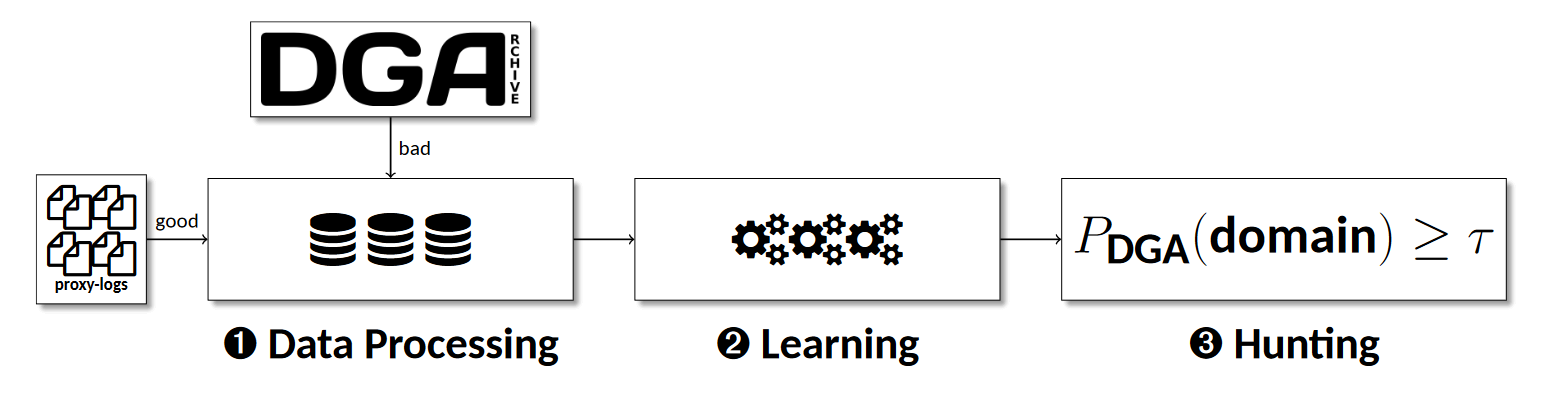
\includegraphics[width=\textwidth]{images/DGA_Detect_Architecture.png}
    \caption{Graphic provided by Tammo Kr\"uger}
    \label{fig:architecture}
\end{figure}\\
During the prototyping phase, I will use a dataset of the top 1 million domains
\cite{noauthor_cisco_nodate} for benign data and
generate AGDs through reverse engineered DGAs \cite{bader_baderjdomain_generation_algorithms_2024}
as malicious data, this will be the dataset during the prototyping phase, during evaluation and
after finalizing the thesis I will try to work with real data from the
DGArchive\cite{dgarchive_2024} and real data from
network traffic to test outside of a "lab setting".~(1)\\
Using these labels we then learn a recurrent neural network, as shown in Figure \ref{fig:RNNLanguageModel},
more specifically a gated recurrent unit, a long short-term memory network with gating mechanism.
Instead on a word level however this network will work on character basis to predict the next
character in the sequence.
Additionally we are use the output of the hidden layers to feed the semantic meaning into a feed
forward network to classify the input, as shown in Chapter 9 of the book \textit{Speech and Language
Processing} by Jurafsky and Martin \cite{jurafsky_speech_nodate}. (2)\\ 
After training the language model the next step is to generate regular expressions. This will be
done by using the distribution output by our model after classifying the domain input. The current
idea is to use specific probability thresholds to determine what RegEx atoms will be generated for
each position in the resulting expression. (3)
\begin{figure}[h]
    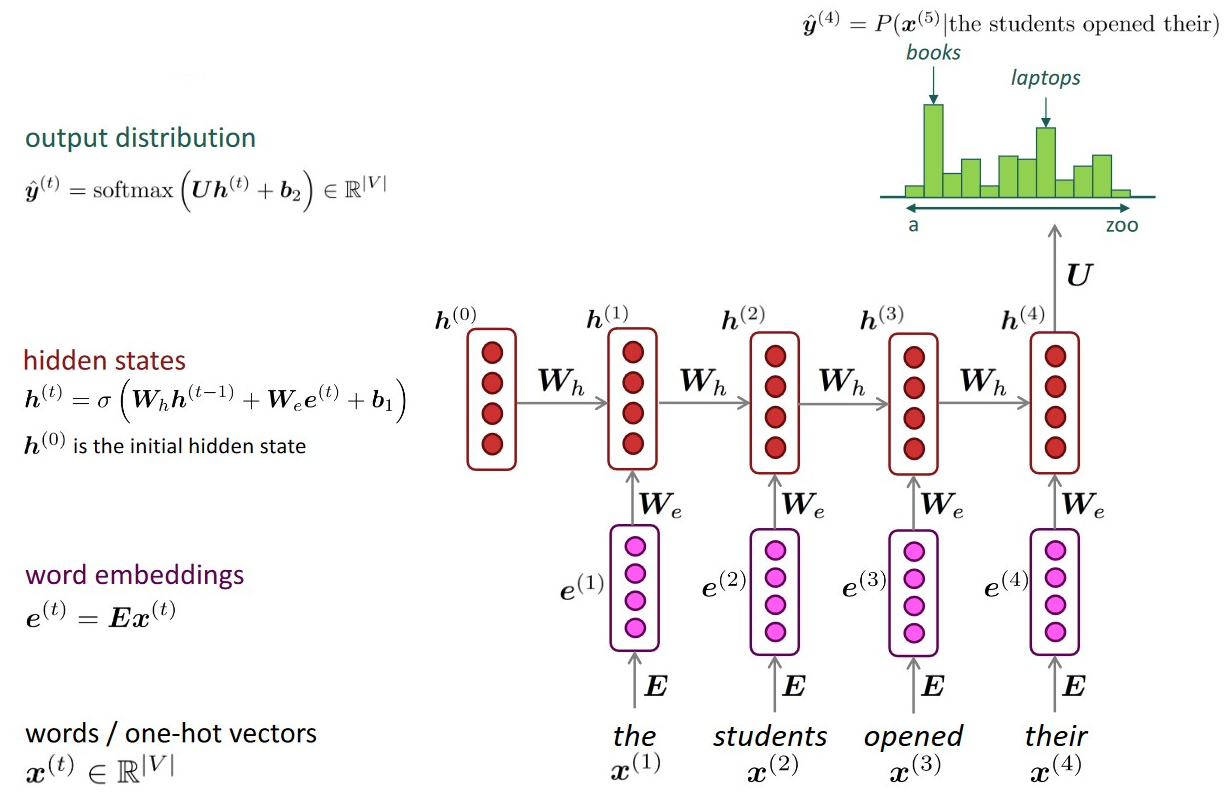
\includegraphics[width=\textwidth]{cs224n-spr2024-lecture05-language-model.png}
    \caption{Example of a RNN Language Model by \cite{manning_natural_2024}}
    \label{fig:RNNLanguageModel}
\end{figure}
\section{Evaluation}
%How is the degree of success of the applied method measured?
I will evaluate the result of this thesis by testing how well the generated regular expressions
will capture the learned structures of DGAs.  It is imperative that however the amount of false
positives (benign domains detected as AGDs) should be very low to not block valid connections with
the generated filter.
The experiment will be set up the following way:\\
The test dataset will be constructed from DGArchive\cite{dgarchive_2024} as the source of AGDs and
real network data will be used for the benign domains.
Using the dataset I will compare the language model and the RegEx to models provided by Yu et al. 
\cite{yu_character_2018}. The evaluation will compare Precision, Recall,
$F_1$-score and area under the ROC curve (AUC), between the character based models, my own language
model and the generated regular expression(s).
During evaluation it is also important that false positive rate is kept low to avoid benign domains
getting blocked.
\section{Scope}
%What is the particular scope of your research? Which goals should be achieved?
%Which are optional and which are explicitly not part of the scope of this
%thesis?
The main scope of this work is determining the possibility of using the generated regular
expressions for filtering and how well it performs compared to my language model and the state of the art.
Part of the necessary work is training a multi-task criterion for the language model and the
classification of DGA and benign domains. 
Once the classification works well the resulting RegEx should detect the learned DGA-families
correctly. Generating easily readable or efficient RegEx, so using specific counts and explicit
character tokens like [abc]\{1,4\} instead of .*, would be a good quality to have but is not
the main focus of this thesis. 
The resulting RegEx also does not need to be better than the current state of the art in detecting
DGAs just have a close enough performance since feasibility of the approach is the main focus of
this thesis.

\section{Related Work}
%Describe the state of the art of the field of research. Support your statements
%with appropriate sources.
The current state of the art in the field are Convolutional Neural Networks and Recurrent Neural
Networks which are also commonly used in Natural Language Processing. Yu et al.
\cite{yu_character_2018} showed that all these approaches achieved similar accuracy and performance
in detecting DGAs.  The paper used the Bambenek dataset for AGDs and the Alexa Dataset for benign
domains. The models were two pure RNN based Architectures (Endgame, CMU), two CNN based
architectures (NYU, Invincea) and one hybrid CNN/RNN based architecture (MIT). 
These models will also be used to compare the results of my model vs. the current state of the art.

\clearpage

\printbibliography

\end{document}
